\section{La idea de Feynman y la construcción del propagador}

    En una fiesta en la taberna Nassau de Princeton, en la primavera de 1941, un físico visitante llamado Herbert Jehle le preguntó a Feynman en qué andaba trabajando. Feynman le contó que estaba buscando una formulación de la mecánica cuántica construida sobre el lagrangiano y no sobre el hamiltoniano, y Jehle le respondió que eso ya estaba hecho, que Dirac había escrito un artículo sobre el asunto. A la mañana siguiente fueron juntos a la biblioteca, encontraron el trabajo de 1933 \citep{dirac1933lagrangian}, y Feynman leyó la frase que lo cambiaría todo: la amplitud de transición en un intervalo infinitesimal \textit{corresponde} a la exponencial de la acción dividida por $\hbar$. Feynman le preguntó a Jehle qué quería decir Dirac con la palabra corresponde, y Jehle contestó que los físicos ingleses la usaban vagamente. Feynman decidió averiguar, allí mismo y en el pizarrón, si corresponde no querría decir simplemente que son iguales salvo una constante. Descubrió que sí. Jehle, según el propio Feynman, se puso a tomar notas frenéticamente \citep{feynman1966development}.

    Lo que salió de esa mañana es el objeto que este capítulo usa para describir la propagación de los fotones. En el capítulo dedicado a la mecánica analítica ya obtuvimos la integral de camino por la vía corta, insertando relaciones de completitud dentro del operador de evolución, y allí nos limitamos a citar el prefactor sin deducirlo. Vale la pena rehacer el camino como lo recorrió Feynman, es decir, empezando por un experimento de interferencia y terminando en una fórmula, porque ese recorrido usa únicamente mecánica clásica, integrales gaussianas y series de Fourier, y porque al final nos dejará el prefactor calculado y no citado.

    \subsection{De la doble rendija a la suma sobre caminos}

        El punto de partida es el experimento más simple que exhibe comportamiento cuántico. Una fuente emite partículas hacia una pantalla con dos rendijas, y detrás hay un detector en el punto $b$. Si solo está abierta la rendija $1$, el detector registra una distribución $P_{1}$; si solo está abierta la $2$, registra $P_{2}$; y con ambas abiertas no registra $P_{1}+P_{2}$ sino un patrón de franjas. La regla que reproduce lo observado, y que en el capítulo de los postulados escribimos como regla de Born, consiste en asociar a cada alternativa un número complejo, sumar los números y elevar al cuadrado el módulo de la suma,
        \begin{equation}\label{eq:DosRendijas}
            \phi = \phi_{1} + \phi_{2}, \qquad P = \left|\phi_{1}+\phi_{2}\right|^{2} \neq \left|\phi_{1}\right|^{2} + \left|\phi_{2}\right|^{2} .
        \end{equation}
        El término cruzado que sobra al desarrollar el módulo al cuadrado es la interferencia, y todo el contenido del experimento está en que las amplitudes se suman antes de elevarse al cuadrado y no después.

        El salto de Feynman consiste en preguntarse qué ocurre si perforamos más agujeros. Con tres rendijas la amplitud es $\phi = \phi_{1}+\phi_{2}+\phi_{3}$, y con un número arbitrario de ellas
        \begin{equation}\label{eq:MuchasRendijas}
            \phi = \sum_{h} \phi_{h},
        \end{equation}
        donde el índice recorre los agujeros. Si ahora los agujeros se hacen tan numerosos y tan juntos que la pantalla desaparece, la suma se convierte en una integral sobre la posición $x$ en el plano de la pantalla, y el resultado debe ser el mismo que si la pantalla nunca hubiera estado allí, porque una pantalla con infinitos agujeros no es una pantalla.

        El paso siguiente es el que decide el asunto. Con dos pantallas en lugar de una, cada una con sus agujeros, la partícula debe atravesar un agujero de la primera y otro de la segunda para llegar al detector, y como esas son alternativas distintas, sus amplitudes se suman,
        \begin{equation}\label{eq:DosPantallas}
            \phi = \sum_{h_{1}}\sum_{h_{2}} \phi_{h_{1}h_{2}} .
        \end{equation}
        Con $N$ pantallas tendremos $N$ sumas encajadas, y si volvemos a hacer los agujeros infinitamente numerosos en cada una y las pantallas infinitamente numerosas a lo largo del camino, cada sumando queda especificado por la lista de puntos por los que la partícula pasó en cada instante intermedio. Pero una lista de posiciones, una por cada instante, es precisamente lo que en mecánica clásica llamamos una trayectoria. Hemos llegado, sin postular nada, al enunciado que da nombre al método: \textbf{la amplitud total es la suma de las amplitudes de todos los caminos concebibles que unen el punto de partida con el de llegada}, incluidos los que ningún cuerpo clásico recorrería jamás.

        Queda por decir cuánto vale la amplitud de cada camino, y aquí es donde Feynman postula que todos los caminos contribuyen con el mismo módulo y difieren únicamente en la fase, y que esa fase es la acción del camino medida en unidades de $\hbar$,
        \begin{equation}\label{eq:PostuladoFeynman}
            \phi[x(s)] = \text{const}\times \exp\left\{\frac{i}{\hbar}S[x(s)]\right\},
            \qquad
            S[x(s)] = \int_{0}^{t} L\left(x,\dot{x}\right) ds .
        \end{equation}

        Que el módulo sea el mismo para todos es una hipótesis de simetría razonable, pues no hay nada que distinga a un camino de otro salvo su forma. Que la fase sea la acción, en cambio, no es arbitrario y puede argumentarse desde la mecánica clásica, que es lo que nos interesa. Si la fase fuese una funcional cualquiera $\Phi[x]$ del camino, podríamos determinarla así. Cuando el sistema es macroscópico sabemos cuál debe ser el resultado, a saber, que la partícula sigue la trayectoria que hace estacionaria la acción; y la única manera de que una suma de números complejos de módulo igual reproduzca ese resultado es que las fases de los caminos vecinos al clásico coincidan entre sí, es decir, que $\Phi$ sea estacionaria exactamente donde lo es $S$. La elección más simple compatible con esa exigencia es que $\Phi$ sea proporcional a $S$, y la constante de proporcionalidad debe tener dimensiones inversas a las de la acción para que la fase sea un número puro. En la naturaleza solo hay una constante con dimensiones de acción, de modo que $\Phi = S/\hbar$.

        El mecanismo por el cual esa suma reproduce la mecánica clásica es puramente geométrico. Tomemos dos caminos vecinos, uno el clásico y otro que se aparta de él en una cantidad pequeña. Sus acciones difieren, y sus contribuciones a la suma son dos números complejos de igual módulo cuyas fases difieren en $\Delta S/\hbar$. Si esa diferencia de fase es grande comparada con $2\pi$, los dos números apuntan en direcciones esencialmente aleatorias y al sumarse se cancelan; si es pequeña, apuntan casi en la misma dirección y se refuerzan. Con números: para un grano de polvo de un miligramo que se mueve un centímetro en un segundo, la acción es del orden de
        \begin{equation}\label{eq:EstimacionClasica}
            S \sim m v L \sim \left(10^{-6}\,\mathrm{kg}\right)\left(10^{-2}\,\mathrm{m\,s^{-1}}\right)\left(10^{-2}\,\mathrm{m}\right) = 10^{-10}\,\mathrm{J\,s},
        \end{equation}
        que en unidades de $\hbar\approx 10^{-34}\,\mathrm{J\,s}$ vale unos $10^{24}$ radianes. Desviar el camino en una millonésima de milímetro cambia la acción en una parte minúscula, pero esa parte minúscula sigue siendo del orden de $10^{15}$ radianes, de manera que la contribución del camino desviado apunta en una dirección completamente arbitraria respecto de la del camino original. La cancelación es feroz, y solo sobrevive la vecindad del camino para el cual la acción es estacionaria, porque allí, y solo allí, la acción no cambia a primer orden y las fases vecinas coinciden. Para un electrón atado a un átomo, en cambio, la acción típica es del orden de $\hbar$ mismo, no hay cancelación, y todos los caminos cuentan. En esta observación está contenida la respuesta a la objeción que se le hizo a Fermat en el siglo XVII: la luz no escoge el camino de tiempo estacionario, los recorre todos, y el camino estacionario es simplemente aquel cuyos vecinos no lo cancelan.

        Para convertir lo anterior en una fórmula usable necesitamos una definición y una propiedad. La definición es la del \textit{propagador} o núcleo, que es la amplitud de que una partícula que estaba en $x_{I}$ en el instante cero sea hallada en $x_{F}$ en el instante $t$, y que escribimos $K(x_{F},t;x_{I},0)$. Con ella, el conocimiento de la función de onda en un instante determina la de cualquier otro instante, porque las alternativas se suman y el punto de partida es una alternativa más,
        \begin{equation}\label{eq:EvolucionK}
            \psi(x_{F},t) = \int_{\mathbb{R}} K(x_{F},t;x_{I},0)\,\psi(x_{I},0)\,dx_{I} .
        \end{equation}
        Esta expresión es la razón por la cual el propagador nos interesa aquí: tiene exactamente la forma de una integral de difracción, con el núcleo haciendo el papel del factor de propagación y la función de onda inicial el de la amplitud en el plano del objeto. Que esa semejanza sea una coincidencia formal o algo más profundo es el asunto del resto del capítulo.

        La propiedad que necesitamos es la ley de composición. Si la partícula va de $a$ a $b$ pasando por un instante intermedio, debe pasar por algún punto $x_{c}$ en ese instante, y como pasar por un punto o por otro son alternativas mutuamente excluyentes, mientras que recorrer el primer tramo y luego el segundo son sucesos consecutivos, las amplitudes de los tramos se multiplican y las de los puntos intermedios se suman,
        \begin{equation}\label{eq:Composicion}
            K(x_{F},t_{2};x_{I},t_{0}) = \int_{\mathbb{R}} K(x_{F},t_{2};x_{c},t_{1})\,K(x_{c},t_{1};x_{I},t_{0})\,dx_{c} .
        \end{equation}
        Nótese que \eqref{eq:Composicion} no es un postulado adicional sino una consecuencia directa de la suma sobre caminos: partir el conjunto de todos los caminos según el punto por el que cruzan un instante dado, y sumar primero dentro de cada grupo y después sobre los grupos, es simplemente reordenar la suma. La acción, por su parte, se parte igual de bien, pues es una integral en el tiempo y $S_{\text{total}} = S_{\text{primer tramo}} + S_{\text{segundo tramo}}$, de modo que la exponencial del total es el producto de las exponenciales.

        Podemos ahora aplicar \eqref{eq:Composicion} $N$ veces, dividiendo el intervalo $[0,t]$ en $N$ tramos iguales de duración
        \begin{equation}\label{eq:Epsilon}
            \varepsilon = \frac{t}{N},
            \qquad
            t_{j} = j\varepsilon,
            \qquad
            x_{j} = x(t_{j}),
        \end{equation}
        con $x_{0}=x_{I}$ y $x_{N}=x_{F}$ fijos. Componiendo tramo a tramo,
        \begin{equation}\label{eq:Rodajas}
            K(x_{F},t;x_{I},0) = \int\cdots\int \prod_{j=1}^{N-1}dx_{j}\;\prod_{j=0}^{N-1} K\left(x_{j+1},t_{j+1};x_{j},t_{j}\right),
        \end{equation}
        y ahora cada factor se refiere a un intervalo infinitesimal, que es donde el postulado \eqref{eq:PostuladoFeynman} puede aplicarse sin ambigüedad. En un tramo tan corto la partícula no tiene tiempo de hacer nada complicado, de manera que su velocidad puede tomarse constante e igual al cociente incremental y el potencial puede evaluarse en el extremo del tramo,
        \begin{equation}\label{eq:AccionTramo}
            S_{j} = \int_{t_{j}}^{t_{j+1}} L\,ds \approx \varepsilon\left[\frac{m}{2}\left(\frac{x_{j+1}-x_{j}}{\varepsilon}\right)^{2} - V(x_{j})\right],
        \end{equation}
        con un error de orden $\varepsilon^{2}$ que desaparece en el límite. El propagador infinitesimal es entonces
        \begin{equation}\label{eq:NucleoCorto}
            K\left(x_{j+1},t_{j+1};x_{j},t_{j}\right) = \frac{1}{A}\exp\left\{\frac{i\varepsilon}{\hbar}\left[\frac{m}{2}\left(\frac{x_{j+1}-x_{j}}{\varepsilon}\right)^{2} - V(x_{j})\right]\right\},
        \end{equation}
        donde $A$ es la constante de normalización que Dirac había dejado sin determinar y que vamos a calcular ahora.

    \subsection{La constante de normalización y la partícula libre}

        La manera más económica de fijar $A$ consiste en exigir que la ley de composición \eqref{eq:Composicion} se cumpla, porque esa ley no admite constantes sobrantes. Hagámoslo con la partícula libre, para la cual $V=0$, y compongamos dos tramos de duración $\varepsilon$ para ver si el resultado tiene la forma de un solo tramo de duración $2\varepsilon$.

        Antes necesitamos una integral que usaremos sin descanso a lo largo de todo el cálculo. Se trata de la integral gaussiana con exponente imaginario, llamada integral de Fresnel, cuyo valor es
        \begin{equation}\label{eq:Fresnel}
            \int_{-\infty}^{\infty} e^{i a u^{2}}\,du = \sqrt{\frac{i\pi}{a}}\,,
            \qquad a \in \mathbb{R}\setminus\{0\},
        \end{equation}
        y que se obtiene de la gaussiana ordinaria $\int e^{-\beta u^{2}}du = \sqrt{\pi/\beta}$ por continuación analítica, sustituyendo $\beta = -ia$ y entendiendo el resultado como el límite de una gaussiana con parte real positiva infinitesimal, que es lo que garantiza la convergencia. La raíz de $i$ vale $e^{i\pi/4}$, de modo que la integral de Fresnel no es más que una gaussiana con un desfase de un octavo de vuelta.

        Vamos a componer los dos tramos. Escribiendo $x_{0}$, $x_{1}$ y $x_{2}$ para los tres puntos y usando \eqref{eq:NucleoCorto} con $V=0$,
        \begin{equation}\label{eq:ComposicionLibre1}
            K_{2} = \frac{1}{A^{2}}\int_{-\infty}^{\infty}\exp\left\{\frac{im}{2\hbar\varepsilon}\left[\left(x_{2}-x_{1}\right)^{2} + \left(x_{1}-x_{0}\right)^{2}\right]\right\}dx_{1},
        \end{equation}
        y todo el trabajo consiste en hacer esa integral, que es gaussiana en la variable intermedia. Desarrollemos el corchete agrupando las potencias de $x_{1}$,
        \begin{equation}\label{eq:ComposicionLibre2}
            \left(x_{2}-x_{1}\right)^{2} + \left(x_{1}-x_{0}\right)^{2}
            = 2x_{1}^{2} - 2x_{1}\left(x_{0}+x_{2}\right) + x_{0}^{2} + x_{2}^{2},
        \end{equation}
        y completemos el cuadrado en $x_{1}$ sumando y restando el término que hace falta,
        \begin{equation}\label{eq:ComposicionLibre3}
            2x_{1}^{2} - 2x_{1}\left(x_{0}+x_{2}\right)
            = 2\left[x_{1}^{2} - x_{1}\left(x_{0}+x_{2}\right) + \textcolor{blue}{\frac{\left(x_{0}+x_{2}\right)^{2}}{4}}\right] - \textcolor{blue}{\frac{\left(x_{0}+x_{2}\right)^{2}}{2}}
            = 2\left[x_{1}-\frac{x_{0}+x_{2}}{2}\right]^{2} - \frac{\left(x_{0}+x_{2}\right)^{2}}{2},
        \end{equation}
        donde los dos términos en azul se han introducido a propósito y su contribución neta es nula. Los términos que ya no dependen de $x_{1}$ salen fuera de la integral, y lo que queda dentro es exactamente la integral de Fresnel \eqref{eq:Fresnel} con $a = m/\hbar\varepsilon$,
        \begin{equation}\label{eq:ComposicionLibre4}
            \int_{-\infty}^{\infty}\exp\left\{\frac{im}{\hbar\varepsilon}\left[x_{1}-\frac{x_{0}+x_{2}}{2}\right]^{2}\right\}dx_{1} = \sqrt{\frac{i\pi\hbar\varepsilon}{m}} = \sqrt{\frac{2\pi i\hbar\varepsilon}{2m}} .
        \end{equation}
        Reuniendo los factores de fuera, y usando que
        \begin{equation}\label{eq:ComposicionLibre5}
            x_{0}^{2}+x_{2}^{2} - \frac{\left(x_{0}+x_{2}\right)^{2}}{2} = \frac{2x_{0}^{2}+2x_{2}^{2}-x_{0}^{2}-2x_{0}x_{2}-x_{2}^{2}}{2} = \frac{\left(x_{2}-x_{0}\right)^{2}}{2},
        \end{equation}
        el resultado de componer los dos tramos es
        \begin{equation}\label{eq:ComposicionLibre6}
            K_{2} = \frac{1}{A^{2}}\sqrt{\frac{\pi i\hbar\varepsilon}{m}}\;\exp\left\{\frac{im\left(x_{2}-x_{0}\right)^{2}}{2\hbar\left(2\varepsilon\right)}\right\} .
        \end{equation}

        Este es el punto que decide la constante. La exponencial de \eqref{eq:ComposicionLibre6} es exactamente la de un único tramo de duración $2\varepsilon$, tal como exige la ley de composición, de manera que el postulado de Feynman pasa la prueba sin necesidad de ajustar nada. Para que también el prefactor tenga la forma de un solo tramo, es decir, para que sea el mismo $1/A$ pero con $\varepsilon$ reemplazado por $2\varepsilon$, hace falta que
        \begin{equation}\label{eq:CondicionA}
            \frac{1}{A^{2}(\varepsilon)}\sqrt{\frac{\pi i \hbar \varepsilon}{m}} = \frac{1}{A(2\varepsilon)},
        \end{equation}
        y basta probar con $A(\varepsilon) = C\sqrt{\varepsilon}$ para ver que la condición se satisface si $C = \sqrt{2\pi i\hbar/m}$. La constante de normalización queda así determinada,
        \begin{equation}\label{eq:ConstanteA}
            A(\varepsilon) = \sqrt{\frac{2\pi i\hbar\varepsilon}{m}},
        \end{equation}
        y con ella el propagador infinitesimal \eqref{eq:NucleoCorto} está completamente especificado. Lo que Dirac había llamado \textit{corresponde} era, en efecto, una igualdad, y la constante que faltaba es la de \eqref{eq:ConstanteA}.

        El propagador de la partícula libre para un tiempo finito se obtiene ahora sin esfuerzo, porque el cálculo que acabamos de hacer se repite idéntico en cada composición. Componer dos tramos de duración $\varepsilon$ dio un tramo de duración $2\varepsilon$ con la misma forma funcional; componer ese con otro da uno de duración $3\varepsilon$, y así sucesivamente. Por inducción, tras $N$ composiciones,
        \begin{equation}\label{eq:PropagadorLibre}
            K_{\text{libre}}(x_{F},t;x_{I},0) = \sqrt{\frac{m}{2\pi i\hbar t}}\;\exp\left\{\frac{im\left(x_{F}-x_{I}\right)^{2}}{2\hbar t}\right\},
        \end{equation}
        que es un resultado exacto y no una aproximación, porque el error de orden $\varepsilon^{2}$ que cometimos en \eqref{eq:AccionTramo} se anula cuando el potencial es nulo.

        Merece atención el exponente de \eqref{eq:PropagadorLibre}. La trayectoria clásica de una partícula libre que va de $x_{I}$ a $x_{F}$ en un tiempo $t$ es la recta recorrida con velocidad constante $v = (x_{F}-x_{I})/t$, y su acción vale
        \begin{equation}\label{eq:AccionLibre}
            S_{\mathrm{cl}} = \int_{0}^{t}\frac{m}{2}v^{2}\,ds = \frac{m}{2}\frac{\left(x_{F}-x_{I}\right)^{2}}{t^{2}}\,t = \frac{m\left(x_{F}-x_{I}\right)^{2}}{2t},
        \end{equation}
        de manera que \eqref{eq:PropagadorLibre} se lee $K = \sqrt{m/2\pi i\hbar t}\,e^{iS_{\mathrm{cl}}/\hbar}$. La suma sobre infinitos caminos ha dado como resultado la exponencial de la acción de uno solo de ellos, el clásico, multiplicada por un factor que no depende de los extremos. Esto no es una casualidad ni es exclusivo de la partícula libre, y la sección siguiente explica por qué.

    \subsection{Sistemas cuadráticos y el propagador del oscilador}

        Supongamos que el lagrangiano es un polinomio de grado dos en la posición y la velocidad, que es el caso de la partícula libre, del oscilador armónico y de la partícula en un campo uniforme. Podemos separar cada camino en el clásico más una desviación que se anula en los extremos, puesto que todos los caminos comparten los mismos puntos inicial y final,
        \begin{equation}\label{eq:SeparacionCamino}
            x(s) = x_{\mathrm{cl}}(s) + y(s),
            \qquad y(0)=y(t)=0 .
        \end{equation}
        Al sustituir en la acción y desarrollar, aparecen tres tipos de términos: los que no contienen $y$, que reconstruyen $S_{\mathrm{cl}}$; los lineales en $y$, que se anulan idénticamente porque la acción es estacionaria sobre el camino clásico, que es el principio de Hamilton del capítulo de mecánica analítica; y los cuadráticos en $y$, que por ser el lagrangiano de grado dos no dependen ya de $x_{\mathrm{cl}}$. Es decir,
        \begin{equation}\label{eq:AccionSeparadaFey}
            S[x] = S_{\mathrm{cl}} + \textcolor{red}{\left(\text{términos lineales en } y\right)} + S_{2}[y] = S_{\mathrm{cl}} + S_{2}[y],
        \end{equation}
        donde el término marcado en rojo se anula por la estacionariedad. Como los extremos de $y$ están fijos en cero, sumar sobre todos los caminos $x$ equivale a sumar sobre todas las desviaciones $y$, y el factor $e^{iS_{\mathrm{cl}}/\hbar}$ sale fuera de esa suma por no depender de la variable de integración. Resulta entonces que
        \begin{equation}\label{eq:FormaCuadratica}
            K(x_{F},t;x_{I},0) = F(t)\,\exp\left\{\frac{i}{\hbar}S_{\mathrm{cl}}(x_{F},t;x_{I},0)\right\},
        \end{equation}
        con un prefactor $F(t)$ que depende del tiempo transcurrido pero no de dónde se empieza ni de dónde se termina. La aproximación semiclásica es exacta para estos sistemas, y el problema de calcular un propagador se parte en dos piezas independientes: una de mecánica clásica pura, que es hallar $S_{\mathrm{cl}}$, y una de integración gaussiana, que es hallar $F(t)$.

        La primera pieza ya la tenemos. En el capítulo de mecánica analítica calculamos la acción clásica del oscilador armónico imponiendo los extremos $q(0)=q_{I}$ y $q(t)=q_{F}$, y el resultado fue
        \begin{equation}\label{eq:AccionOsciladorAqui}
            S_{\mathrm{cl}} = \frac{m\omega}{2}\left[\left(q_{I}^{2}+q_{F}^{2}\right)\cot\omega t - \frac{2q_{I}q_{F}}{\sin\omega t}\right].
        \end{equation}

        La segunda pieza es la que quedó pendiente allí y la que vamos a calcular aquí, y lo haremos con una herramienta que es de mecánica clásica y no de teoría cuántica de campos: los modos normales. La desviación $y(s)$ es una función que se anula en $s=0$ y en $s=t$, exactamente como el desplazamiento de una cuerda sujeta por los dos extremos, de manera que admite un desarrollo en la serie de senos correspondiente,
        \begin{equation}\label{eq:SerieSenos}
            y(s) = \sum_{n=1}^{\infty} a_{n}\sin\left(\frac{n\pi s}{t}\right),
        \end{equation}
        y sumar sobre todos los caminos de desviación equivale a integrar sobre todos los valores posibles de los coeficientes $a_{n}$. Este cambio de variables convierte una integral funcional, que es un objeto incómodo, en un producto de integrales ordinarias, que no lo es.

        En estas variables, $S_{2}[y]$ se calcula sin dificultad. Para el oscilador,
        \begin{equation}\label{eq:S2Oscilador}
            S_{2}[y] = \int_{0}^{t}\left(\frac{m}{2}\dot{y}^{2} - \frac{m\omega^{2}}{2}y^{2}\right)ds,
        \end{equation}
        y necesitamos las dos integrales de los productos de senos y cosenos, que son las relaciones de ortogonalidad de siempre,
        \begin{equation}\label{eq:OrtogonalidadSenos}
            \int_{0}^{t}\sin\left(\frac{n\pi s}{t}\right)\sin\left(\frac{n'\pi s}{t}\right)ds = \frac{t}{2}\delta_{nn'},
            \qquad
            \int_{0}^{t}\cos\left(\frac{n\pi s}{t}\right)\cos\left(\frac{n'\pi s}{t}\right)ds = \frac{t}{2}\delta_{nn'} .
        \end{equation}
        Derivando \eqref{eq:SerieSenos} término a término, $\dot{y} = \sum_{n} a_{n}(n\pi/t)\cos(n\pi s/t)$, y sustituyendo ambas series en \eqref{eq:S2Oscilador}, las deltas de \eqref{eq:OrtogonalidadSenos} colapsan las dobles sumas en sumas simples,
        \begin{equation}\label{eq:S2Diagonal}
            S_{2} = \frac{m}{2}\cdot\frac{t}{2}\sum_{n=1}^{\infty}\left(\frac{n\pi}{t}\right)^{2}a_{n}^{2} - \frac{m\omega^{2}}{2}\cdot\frac{t}{2}\sum_{n=1}^{\infty}a_{n}^{2}
            = \frac{mt}{4}\sum_{n=1}^{\infty}\left[\left(\frac{n\pi}{t}\right)^{2}-\omega^{2}\right]a_{n}^{2} .
        \end{equation}
        La acción de las fluctuaciones ha quedado diagonal: no hay términos cruzados entre modos distintos, y cada coeficiente aparece elevado al cuadrado y multiplicado por un número. Esta es la razón por la cual los modos normales son la variable correcta, y es el mismo motivo por el que lo son en la cuerda vibrante o en la cavidad del capítulo anterior.

        La integral sobre las fluctuaciones se factoriza entonces en un producto de integrales de Fresnel independientes, una por cada modo,
        \begin{equation}\label{eq:ProductoFresnel}
            F(t) = J \prod_{n=1}^{\infty}\int_{-\infty}^{\infty}\exp\left\{\frac{imt}{4\hbar}\left[\left(\frac{n\pi}{t}\right)^{2}-\omega^{2}\right]a_{n}^{2}\right\}da_{n}
            = J\prod_{n=1}^{\infty}\sqrt{\frac{4\pi i\hbar}{mt\left[\left(n\pi/t\right)^{2}-\omega^{2}\right]}},
        \end{equation}
        donde $J$ recoge el jacobiano del cambio de variables entre las posiciones intermedias y los coeficientes $a_{n}$, junto con los factores $1/A$ de la medida. Ese $J$ es incómodo y, tomado por separado, ni siquiera es finito; pero tiene una virtud decisiva, y es que no depende de $\omega$, puesto que el cambio de variables \eqref{eq:SerieSenos} no sabe nada del potencial. Podemos por tanto deshacernos de él comparando el oscilador con la partícula libre, cuyo prefactor ya conocemos de \eqref{eq:PropagadorLibre}. Dividiendo \eqref{eq:ProductoFresnel} por la misma expresión evaluada en $\omega = 0$, el jacobiano se cancela y también lo hacen todos los factores constantes de cada modo,
        \begin{equation}\label{eq:Cociente}
            \frac{F_{\omega}(t)}{F_{0}(t)} = \prod_{n=1}^{\infty}\sqrt{\frac{\left(n\pi/t\right)^{2}}{\left(n\pi/t\right)^{2}-\omega^{2}}}
            = \prod_{n=1}^{\infty}\left[1 - \frac{\omega^{2}t^{2}}{n^{2}\pi^{2}}\right]^{-1/2} .
        \end{equation}

        El producto infinito que ha aparecido es conocido desde Euler. Se trata de la factorización del seno en términos de sus ceros,
        \begin{equation}\label{eq:ProductoEuler}
            \frac{\sin z}{z} = \prod_{n=1}^{\infty}\left(1 - \frac{z^{2}}{n^{2}\pi^{2}}\right),
        \end{equation}
        que puede entenderse sin dificultad: el miembro derecho se anula exactamente en $z = \pm n\pi$, que son los ceros del seno distintos del origen, y vale uno en $z=0$, igual que el izquierdo. Identificando $z = \omega t$, el producto de \eqref{eq:Cociente} es precisamente $\sin(\omega t)/(\omega t)$ elevado a la potencia $-1/2$, de manera que
        \begin{equation}\label{eq:CocienteFinal}
            \frac{F_{\omega}(t)}{F_{0}(t)} = \sqrt{\frac{\omega t}{\sin\omega t}} .
        \end{equation}
        Sustituyendo el prefactor libre $F_{0}(t) = \sqrt{m/2\pi i\hbar t}$, los dos factores de $t$ se cancelan y queda
        \begin{equation}\label{eq:PrefactorOscilador}
            F_{\omega}(t) = \sqrt{\frac{m}{2\pi i\hbar t}}\sqrt{\frac{\omega t}{\sin\omega t}} = \sqrt{\frac{m\omega}{2\pi i\hbar\sin\omega t}} .
        \end{equation}

        Reuniendo \eqref{eq:AccionOsciladorAqui} y \eqref{eq:PrefactorOscilador} en la forma general \eqref{eq:FormaCuadratica} obtenemos el propagador del oscilador armónico,
        \begin{equation}\label{eq:PropagadorOsciladorFeynman}
            K(q_{F},t;q_{I},0) = \left(\frac{m\omega}{2\pi i\hbar\sin\omega t}\right)^{1/2}
            \exp\left\{\frac{i m\omega}{2\hbar}\left[\left(q_{I}^{2}+q_{F}^{2}\right)\cot\omega t - \frac{2q_{I}q_{F}}{\sin\omega t}\right]\right\},
        \end{equation}
        deducido sin más herramientas que la suma sobre caminos, el principio de Hamilton, unas integrales gaussianas y una serie de Fourier.

        Antes de seguir podemos verificar dos límites. Cuando la frecuencia tiende a cero, usando $\sin\omega t\to\omega t$ y $\cot\omega t\to 1/\omega t$, el prefactor tiende a $\sqrt{m/2\pi i\hbar t}$ y el exponente a $im(q_{I}^{2}+q_{F}^{2}-2q_{I}q_{F})/2\hbar t$, que es la partícula libre \eqref{eq:PropagadorLibre}, como debía ser. Cuando $\omega t$ se acerca a un múltiplo de $\pi$, en cambio, el prefactor diverge, y esa divergencia no es un defecto del cálculo sino un hecho físico: transcurrido medio período todas las trayectorias que salieron de $q_{I}$ vuelven a reunirse en el mismo punto, de modo que la amplitud se concentra allí. Son los puntos conjugados que ya encontramos al calcular la acción clásica, y su análogo óptico es el foco de un sistema formador de imagen.

        Queda por decir cómo se conecta esto con el fotón, que es de lo que trata el capítulo. En el capítulo dedicado a la cuantización vimos que el campo electromagnético encerrado en una cavidad es dinámicamente equivalente a una colección de osciladores armónicos independientes, uno por cada modo, y que las variables canónicas de cada modo están normalizadas de manera que la masa efectiva vale la unidad. Poniendo $m=1$ en \eqref{eq:PropagadorOsciladorFeynman} se obtiene
        \begin{equation}\label{eq:PropagadorModo}
            K(q_{F},t;q_{I},0) = \left(\frac{\omega}{2\pi i\hbar\sin\omega t}\right)^{1/2}
            \exp\left\{\frac{i\omega}{2\hbar}\left[\left(q_{I}^{2}+q_{F}^{2}\right)\cot\omega t - \frac{2q_{I}q_{F}}{\sin\omega t}\right]\right\},
        \end{equation}
        que es exactamente la amplitud de transición de la que parte la sección siguiente. El resto del capítulo consiste en tomar en serio la forma de esta expresión, que combina una fase cuadrática en los dos extremos con un término cruzado, y reconocer en ella el núcleo de una transformada de Fourier fraccionaria y, por tanto, una integral de difracción de Fresnel.

\section{Propagador de fotones}

    En esta parte vamos a abordar la naturaleza de la propagación de los fotones y su relación con el principio de Huygens-Fresnel. Aunque el uso de la fórmula de difracción de Rayleigh-Sommerfeld como propagador de fotones es ampliamente aceptado debido a la evidencia experimental disponible, aún existen interrogantes sobre la conexión directa entre la propagación del campo electromagnético en la óptica clásica y la propagación de los fotones, donde el cuadrado de la amplitud de probabilidad describe la probabilidad transversal de detección del fotón.

    Además, se presenta una formulación matemática para la propagación de los fotones utilizando el formalismo de la cuantización del campo electromagnético y el método de la integral de camino. Esta formulación tiene una similitud destacada con una transformada de Fourier fraccional (FRFT, por sus siglas en inglés). Se demuestra que debido a la estrecha relación existente entre la FRFT y la integral de difracción de Fresnel, este propagador puede expresarse como una difracción de Fresnel, lo que plantea una discusión sobre su carácter fundamental a nivel de fotón en comparación con el principio de Huygens-Fresnel.
    
    Finalmente, se realiza un experimento de conteo de fotones utilizando una rendija rectangular, confirmando que el fenómeno de difracción en la aproximación de Fresnel se comporta de manera similar al límite clásico real.
    \subsection{Propagador de fotón}
    
    La amplitud de transición correspondiente para el Hamiltoniano de un campo electromagnético cuantizado es calculada mediante el método de la integral de trayectoria:
    
    \begin{equation}
        \left < q_{F} \left | e^{-i\hat{H}t/\hbar} \right | q_{I} \right > = \left ( \frac{\omega}{2\pi i \hbar \sin (\omega t)} \right ) ^{\frac{1}{2}} \exp \left \{  \frac{i}{2\hbar}\omega  \left [ \left (  q_{I}^{2}+q_{F}^{2} \right ) \cot (\omega t) - \frac{2q_{I}q_{F}}{\sin (\omega t)} \right ] \right \}
    \end{equation}
    
    Entonces, la evolución temporal de un sistema en un estado $\left | \psi  \right >$ en la representación de $q$ se escribe:
    
    \begin{equation}
        \psi(q_{F},t)= \left ( \frac{\omega}{2\pi i \hbar \sin (\omega t)} \right ) ^{\frac{1}{2}} \int _{\mathbb{R}} \psi (q_{I},0) \exp \left \{  \frac{i}{2\hbar}\omega  \left [ \left (  q_{I}^{2}+q_{F}^{2} \right ) \cot (\omega t) - \frac{2q_{I}q_{F}}{\sin (\omega t)} \right ] \right \} dq_{I}
        \label{propagfoton}
    \end{equation}
    Esta ecuación describe cómo evoluciona en el tiempo la “función de onda” a medida que se propaga la luz, cuyo núcleo se escribe como una transformada de Fourier y una fase cuadrática al igual que la integral de difracción de Fresnel en la propagación clásica del campo electromagnético. Esta similitud nos permite establecer una conexión donde la integral de difracción de Fresnel juega un papel importante en la propagación de fotones.
    
    \subsection{Propagador del campo electromagnético clásico}
    
    La integral de difracción de Fresnel en una dimensión, a una distancia $z$, en el marco de la óptica metaxial de Bonnet se escribe:
    
    \begin{equation}
        U(x,z) = \left ( \frac{i}{\lambda z} \right )^{\frac{1}{2}} e^{ikz} \exp \left [ -\frac{ik}{2}\left ( \frac{1}{z} + \frac{1}{R_{B}}\right )x^{2} \right ]\int_{\Sigma }  \exp \left [ -\frac{ik}{2}\left ( \frac{1}{z} - \frac{1}{R_{A}}\right )x'^{2} \right ] \exp\left [ \frac{ik}{z}xx' \right ] U(x',0) dx'
        \label{eqfresnel}
    \end{equation}
    
    Donde las ondas esféricas se aproximan a parabólicas y el radio de curvatura para $U$ desde su vértice hasta el centro se define como la cantidad algebraica $R_{A} = \overline{VC}$, y se considera positivo si va en la dirección de propagación de la luz. 
    
    \begin{figure}[htbp]
        \centering    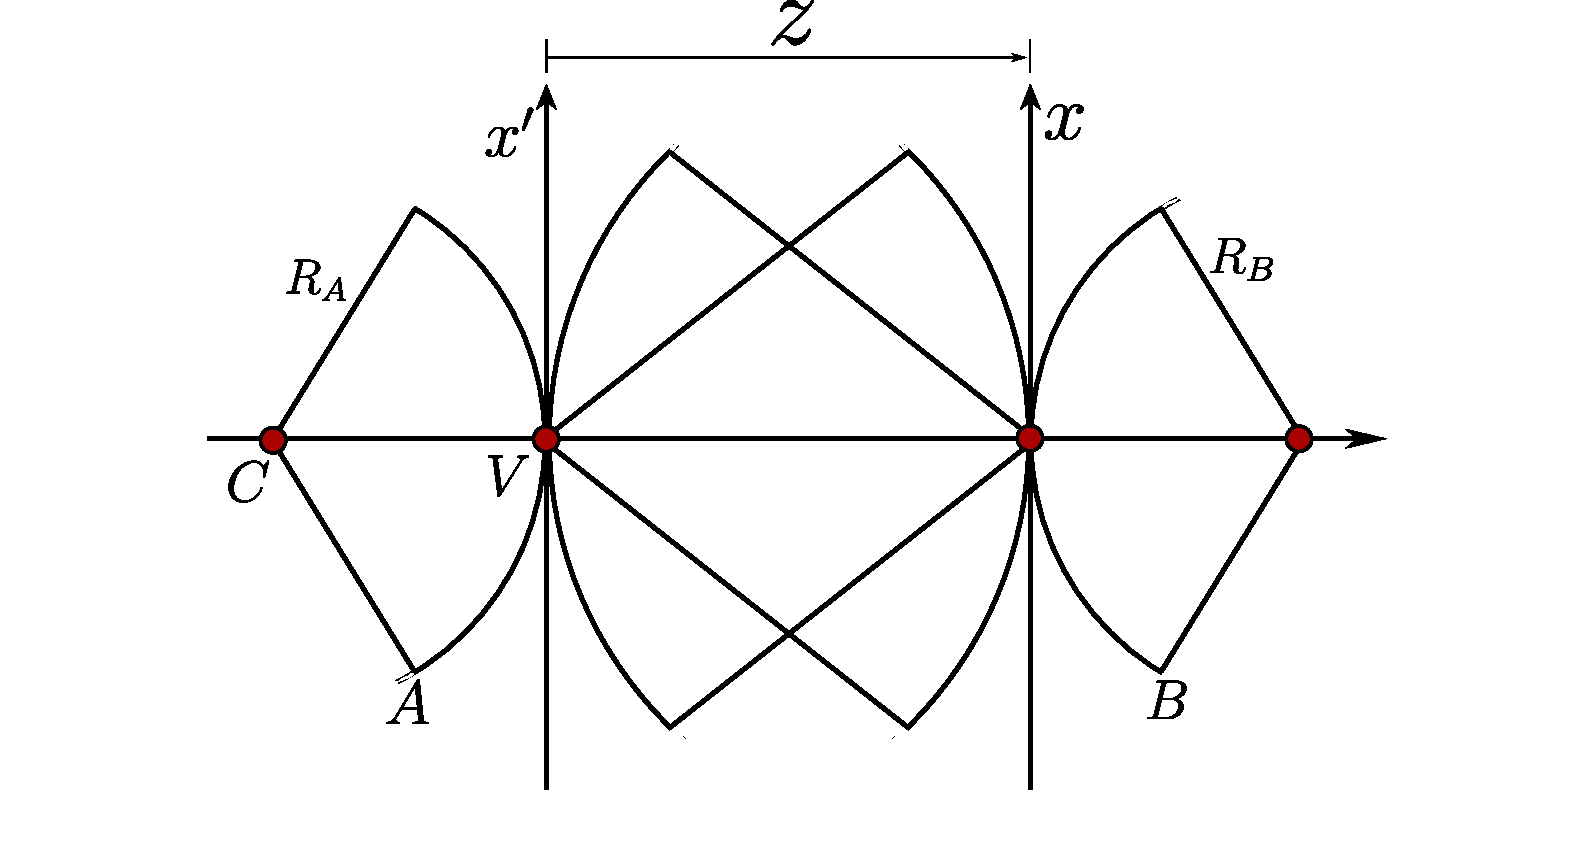
\includegraphics[width=0.9\textwidth]{Capitulo 8/Figuras/difraccionfresnel.pdf}
        \caption{Difracción de Fresnel entre la superficie esférica $A$ y la superficie esférica $B$.}
        \label{fig:difraccionfresnel}
    \end{figure}
    
    Pellat-Finet estableció una relación entre la difracción de Fresnel y la transformación de Fourier fraccionaria. Escribiendo las amplitudes del campo y las variables reducidas:
    
    \begin{equation}
        V_{A}(\rho) = U_{A}(\sqrt{\lambda \varepsilon R_{A}}\rho)\, ,\hspace{0.7cm} 
        V_{B}(\sigma) = U_{B}\left ( \frac{\sqrt{\lambda \varepsilon R_{A}}\sigma}{\cos \alpha + \varepsilon \sin \alpha} \right )
    \end{equation}
    \begin{equation}        
        \rho = \frac{1}{\sqrt{\lambda \varepsilon R_{A}}}x'\, ,\hspace{0.7cm}
        \sigma = \frac{1}{\sqrt{\lambda \varepsilon R_{A}}}(\cos \alpha + \varepsilon \sin \alpha)x
        \label{variablered}
    \end{equation}
    
    Dónde 
    \begin{equation}
        \cot \alpha = \varepsilon \frac{1-\mu}{\mu}\hspace{0.7cm} \mathrm{y} \hspace{0.7cm} \mu = \frac{z}{R_{A}}
        \label{eqcot}
    \end{equation}
    \begin{equation}
        \sin ^{2} \alpha = \frac{\mu ^{2}}{\mu ^{2} + \varepsilon ^{2} (1-\mu)^{2}}
        \label{eqsin}
    \end{equation}
    Además $\varepsilon$ es la solución en número real distinta de cero de:
    
    \begin{equation}
        \frac{1}{R_{B}} + \frac{1}{z} = \frac{\varepsilon^{2}(1-\mu)}{\mu R_{A}[\mu^{2} + \varepsilon^{2}(1-\mu)^{2}]}
        \label{eqradios}
    \end{equation}
    
    La ecuación $\ref{eqfresnel}$ se reescribe de la forma:
    
    \begin{equation}
        V_{B}(\sigma) = \frac{i}{\sin\alpha} (\cos \alpha + \varepsilon \sin \alpha) \int_{\mathbb{R}} V_{A}(\rho) \exp \left [ i\pi (\rho^{2}+ \sigma^{2})\cot \alpha - \frac{2i\pi \sigma \rho}{\sin \alpha} \right ] d\rho
        \label{tffr}
    \end{equation}
    
    Con esto, la relación entre el propagador de fotones $(\ref{propagfoton})$ y la integral de difracción de Fresnel escrita en la forma de la ecuación $\ref{tffr}$ es más clara. Solo se necesita encontrar el factor de escala para las variables reducidas apropiadas para $q_{I}$ y $q_{F}$.
    
    \subsection{Propagación como una integral de Fresnel}
    
    Para establecer una relación entre el propagador $(\ref{propagfoton})$ y la transformada de Fourier fraccionaria, se realiza el siguiente cambio de variables:
    
    \begin{equation}
        \rho^{2} = \frac{\omega}{2 \pi \hbar} q_{I}^{2}\, ,\hspace{0.7cm}
        \sigma^{2} = \frac{\omega}{2 \pi \hbar} q_{F}^{2}
    \end{equation}
    
    Usando $\alpha = wt$, $k = \frac{2\pi}{\lambda}$, $ct=\varepsilon R_{A}>0$ y difiniendo un término de masa $m_{\lambda} = \frac{\hbar k}{c}$ que está relacionado con el Hamiltoniano, es decir, el campo electromagnético cuantizado puede entenderse como un oscilador armónico mecánico cuántico con masa $m_{\lambda}$.
    
    \begin{equation}
        \rho^{2} = \frac{1}{\lambda \varepsilon R_{A}} \frac{\alpha}{m_{\lambda}} q_{I}^{2}\, ,\hspace{0.7cm}
        \sigma^{2} = \frac{1}{\lambda \varepsilon R_{A}} \frac{\alpha}{m_{\lambda}}  q_{F}^{2}
    \end{equation}
    
    Luego, usando las expresiones en $(\ref{variablered})$ se encuentra que la escala entre el observable $q$ y una posición real $x$ es:
    
    \begin{equation}
        x_{I}^{2} = \frac{\alpha}{m_{\lambda}}q_{I}^{2} \, ,\hspace{0.7cm}
        x_{F}^{2} = \frac{\alpha}{m_{\lambda}}q_{F}^{2}
    \end{equation}
    
    Donde 
    \begin{equation}
        \cos \alpha + \varepsilon \sin \alpha = 1
        \label{eqcos}
    \end{equation}
    
    Entonces la ecuación $\ref{propagfoton}$ se puede escribir de la forma:
    
    \begin{equation}
        \Psi(x_{F},t) = \left ( \frac{\omega}{2i\pi \hbar \sin (\omega t)} \right )^{\frac{1}{2}}\left ( \frac{m_{\lambda}}{\alpha} \right ) ^{\frac{1}{2}} \int_{\mathbb{R}} \psi(x_{I},0) \exp \left \{ \frac{i\pi}{\lambda \varepsilon R_{A}} \left [ \left ( x_{I}^{2} + x_{F}^{2} \right ) \cot \alpha - \frac{2 x_{I} x_{F}}{\sin \alpha} \right ]\right \} dx_{I}
        \label{propagador3}
    \end{equation}
    
    Con 
    \begin{equation}
        \Psi(x_{I},0) = \psi \left ( \sqrt{\frac{m_{\lambda}}{\alpha}}x_{I},0 \right ) \hspace{0.7cm} \mathrm{y} \hspace{0.7cm} \Psi(x_{F},t) = \psi \left ( \sqrt{\frac{m_{\lambda}}{\alpha}}x_{F},t \right )
    \end{equation}
    
    Además, usando $\ref{eqcot}$ y $\ref{eqcos}$ se llega a:
    
    \begin{equation}
        \sin \alpha = \frac{\mu}{\varepsilon}
        \label{eqsin2}
    \end{equation}
    
    Entonces, igualando $\ref{eqsin}$ y $\ref{eqsin2}$ se tiene:
    
    \begin{equation}
        \mu ^{2} + \varepsilon ^{2} (1-\mu)^{2} = \varepsilon ^{2}
    \end{equation}
    
    Con $\varepsilon ^{2} = \frac{\mu}{2- \mu}$. Entonces la ecuación $\ref{eqradios}$ toma la forma:
    
    \begin{equation}
        \frac{1}{R_{B}} + \frac{1}{z} = \frac{1-\mu}{\mu R_{A}}
    \end{equation}
    
    Finalmente, teniendo $R_{B} = -R_{A}$ la expresión $(\ref{propagador3})$ se puede escribir explícitamente en términos de la posición y la distancia de propagación $z$ como
    
    \begin{equation}
        \psi(x_{F},z) = \left ( \frac{i}{\lambda z} \right )^{\frac{1}{2}} \exp \left [ -\frac{ik}{2} \left ( \frac{1}{z} + \frac{1}{R_{B}} \right ) x_{F}^{2}  \right ] \int_{\Sigma} \exp \left [ -\frac{ik}{2} \left ( \frac{1}{z} - \frac{1}{R_{A}} \right ) x_{I}^{2}  \right ] \exp \left [ \frac{ik}{z} x_{I} x_{F} \right ] \psi (x_{I},0) dx_{I}
        \label{eq:fresnelclasica}
    \end{equation}
    
    La cual, es exactamente la fórmula clásica de difracción de Fresnel eliminando el factor de fase $e^{ikz}$. Además, se puede escribir en términos de las variables reducidas $\rho$ y $\sigma$ como la transformada de Fourier fraccionaria,
    
    \begin{equation}
        \phi (\sigma) = \left ( \frac{1}{i \sin \alpha} \right )^{\frac{1}{2}} \int_{\mathbb{R}} \exp \left \{ i \pi \left [ \left ( \rho^{2} + \sigma^{2} \right ) \cot \alpha - \frac{2 \rho \sigma}{\sin \alpha} \right ] \right \} \phi (\rho) d \rho
        \label{eq:FRFT}
    \end{equation}
    
    De esta manera, la $FRFT$ expresa matemáticamente la propagación de fotones de la misma forma que se emplea para propagar el campo clásico en el régimen de Fresnel. Se debe tener en cuenta que cuando $\alpha = \frac{\pi}{2}$, la propagación se convierte en la transformada de Fourier estándar (régimen de Fraunhofer). Lo notable aquí es que ahora disponemos de una herramienta ampliamente reconocida para estudiar la propagación de fotones, y podemos aplicar todas las propiedades del análisis de Fourier a la óptica cuántica. \\
    
    Como podemos ver, la función de onda $\Psi(x,t)$ se comporta como una función de onda de campo eléctrico que está estrechamente relacionada por algunos factores de escala con la función de onda $\psi(x,t)$ en la representación $q$ y se puede propagar de la misma manera como la integral de difracción de Fresnel clásica. Dado que en ambos casos —cuántico y clásico— la amplitud de probabilidad y la amplitud del campo eléctrico evolucionan de la misma manera, esto significa que el observable $q$ puede considerarse como una posición en la dirección transversal a la propagación del campo y paralela a la dirección de propagación de polarización del campo eléctrico. \\
    
    Por lo tanto, la ecuación $(\ref{propagfoton})$ representaría la evolución de la amplitud de probabilidad transversal, $\psi(x,t)$, de detectar un fotón, quedando deslocalizado longitudinalmente. Esto significa que el observable $\hat{q}$ está lejos de lo que puede considerarse como la posición del fotón. Vale la pena mencionar que no existe un operador de posición para fotones y no existe una descripción mecánica cuántica satisfactoria para el fotón en el sentido habitual.
    
    
    \subsection{Correspondencia a la teoría de la difracción escalar}
    
    ¿Es posible que la difracción de Fresnel no sea una simple aproximación a la fórmula de Rayleigh-Sommerfeld sino que describa de manera fundamental la propagación del campo de radiación? A continuación se mostrará cómo se puede ajustar la teoría de la difracción escalar para obtener una expresión diferente de un campo propagado. \\
    Se propone que el campo electromagnético no puede estar confinado en una región puntual sino en un pequeño volumen. No es muy instintivo pensar en una fuente puntual para una onda electromagnética o fotones ya que la densidad de energía espacial sería infinita. Por ejemplo, en la Ref. [33], los autores demuestran que las fuentes secundarias de Huygen tienen una dimensión y una densidad de energía finitas; además, se ha demostrado [30] que los fotones no se pueden localizar de forma nítida, aunque se ha estudiado la posibilidad de tener pulsos monofotónicos de área cero [34]. Por lo tanto, consideramos que cualquier fuente de ondas electromagnéticas $U(r,t)$ con longitud de onda $\lambda$ debe tener una amplitud constante en una vecindad de al menos el orden de la longitud de onda. Ahora bien, recordemos que en la teoría escalar de la difracción se utiliza el teorema de Green para calcular la propagación del campo electromagnético [1,2,26]. Se desea resolver, para $U$, la expresión:
    
    \begin{equation}
        \int_{V} U(\nabla ^{2} + k^{2}) G dv = \int_{S} \left ( U \frac{\partial G}{\partial n} - G \frac{\partial U}{\partial n} \right ) ds
        \label{intgreen}
    \end{equation}
    
    dónde $G$ es una función auxiliar, conocida como función de Green.
    
    \begin{equation}
        (\nabla^{2} + k^{2})'G_{\pm}(\vec{r}, \vec{r'}) = -4\pi [\delta(\vec{r} - \vec{r'}) \pm \delta(\vec{r} - \widetilde{\vec{r'}})]
        \label{condgreen}
    \end{equation}
    
    que representa una fuente puntual en $\vec{r'}$ $\in$ $V$ y $\widetilde{\vec{r'}}$ $\notin$ $V$. Esto permite el cálculo del campo $U$ en la región $V$ del espacio a la derecha del plano [Fig. $\ref{ftesferica}$]. Una solución para $G$, en el sentido de distribuciones, corresponde a la onda esférica,
    
    \begin{equation}
        G_{\pm} (\vec{r}, \vec{r'}) = \frac{e^{ik\left | \vec{r} - \vec{r'} \right |}}{\left | \vec{r} - \vec{r'} \right |} \pm \frac{e^{ik\left | \vec{r} - \widetilde{\vec{r'}} \right |}}{\left | \vec{r} - \widetilde{\vec{r'}} \right |}
    \end{equation}
    
    \begin{figure}[htbp]
    \centering
        \subfloat[]{
        \label{ftesferica}
        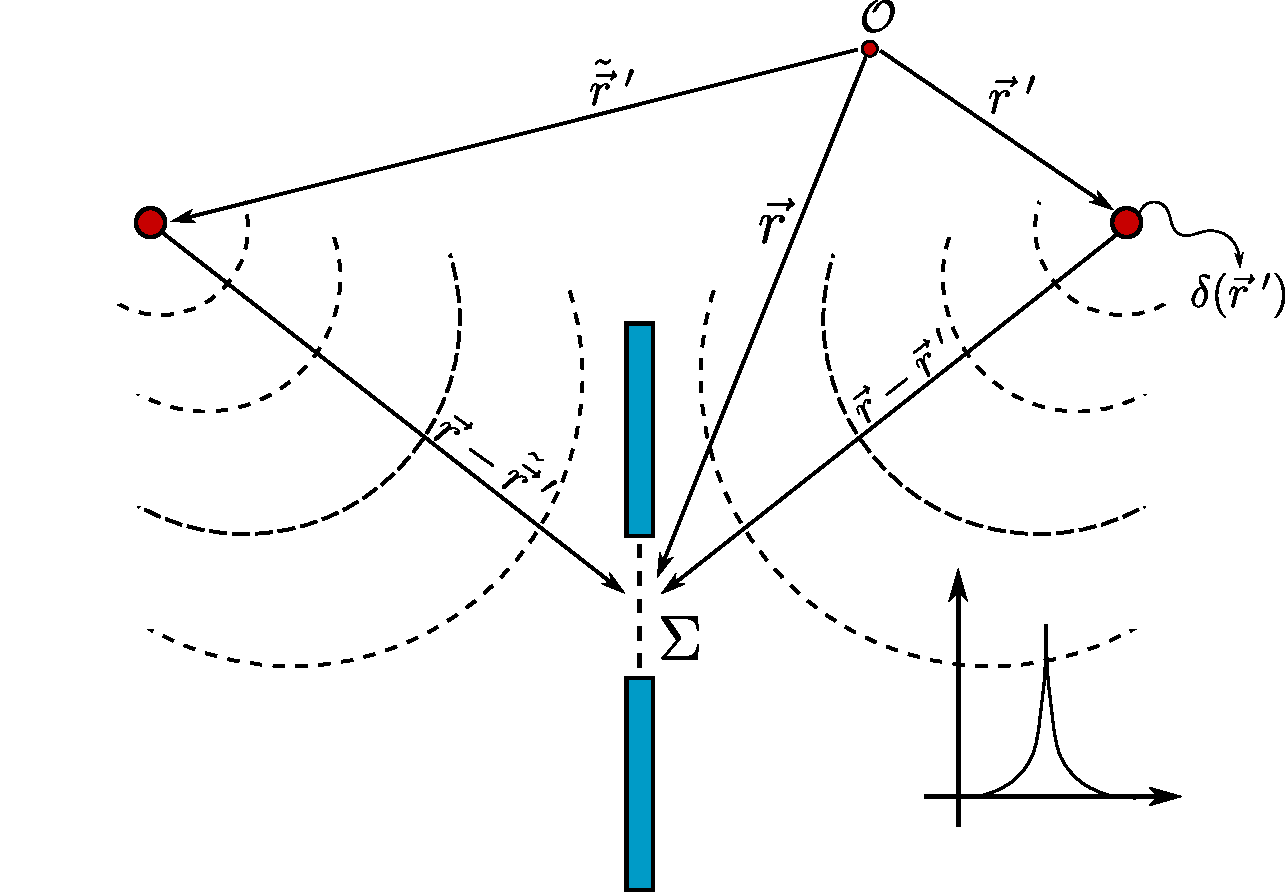
\includegraphics[width=0.5\textwidth]{Capitulo 8/Figuras/ftesferica.pdf}}
        \subfloat[]{
        \label{ftparabol}
        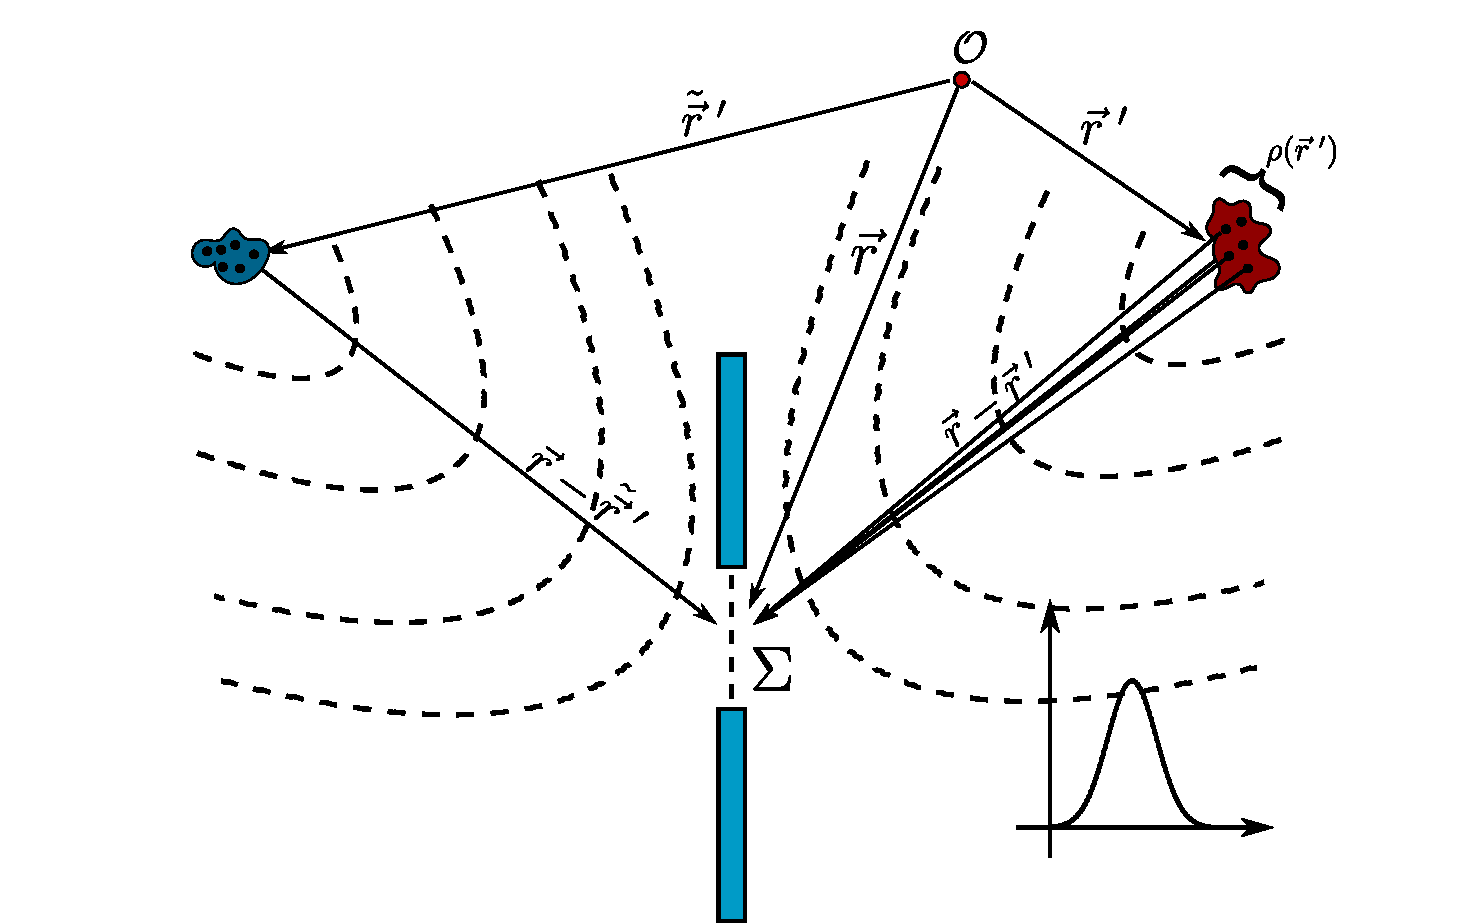
\includegraphics[width=0.5\textwidth]{Capitulo 8/Figuras/ftparabol.pdf}}
    \caption{$(a)$ Problema de Green usando una distribución $\delta$ de Dirac. $(b)$ Problema propuesto para una distribución arbitraria.}
    \label{fuentes}
    \end{figure}
     
    respectivamente, la expresión $\ref{intgreen}$ se reduce a:
    
    \begin{equation}
        U(r) = \frac{1}{4\pi} \int_{\Sigma} U \frac{\partial G_{-}}{\partial n} ds
    \end{equation}
    
    lo que da lugar a la fórmula de Rayleigh-Sommerfeld del principio de Huygens-Fresnel. \\
    Ahora bien, dado que nuestra premisa es que una onda electromagnética no puede definirse en un solo punto, sino distribuirse en una vecindad $v(\vec{r})$ $\subseteq $ $V$ de un punto definido por $\vec{r}$, la distribución de Dirac debe ser reemplazada por otra distribución que nos permita considerar el campo en la vecindad $v(\vec{r})$ como una constante, $U(v(\vec{r})) = U(\vec{r})$ [Fig. $\ref{ftparabol}$]. \\
    
    Por lo tanto, se propone, en lugar de la condición de Green $[Eq. (\ref{condgreen})]$, una nueva condición
    
    \begin{equation}
        (\nabla^{2} + k^{2})'\mathcal{G}_{\pm}(\vec{r}, \vec{r'}) = \rho (\vec{r} - \vec{r'}) \pm \rho(\vec{r} - \widetilde{\vec{r'}})
        \label{condgreen2}
    \end{equation}
    
    donde la expresión
    
    \begin{equation}
        \int_{V} U(\vec{r'}) \underbrace{(\nabla ^{2} + k^{2})' \mathcal{G} _{\pm}}_{\textstyle \rho(\vec{r} - \vec{r'})} dv' = U(v(\vec{r})) = U(\vec{r})
        \label{intgreen2}
    \end{equation}
    
    se mantiene. Recuerde que la integral se calcula en la región $V$ [lado derecho de la figura (\ref{fuentes})], donde la fuente del espejo auxiliar no afecta el resultado. \\
    
    Notemos que si colocamos las fuentes puntuales en pares (uno en la región donde se mide el campo y otro en la imagen especular), un par tras otro hasta formar un cúmulo [Fig. $\ref{ftparabol}$], entonces $\rho$ se puede escribir en base a las distribuciones de Dirac, y se puede elegir que la función $G_{\pm}$ o su derivada sean cero en el plano $(\Sigma)$ que cumpla las condiciones de Dirichlet o Neumann. Es decir, se puede elegir $\mathcal{G}(\Sigma) = 0$ o $\frac{\mathcal{G}}{n} (\Sigma) = 0$, y luego el campo se puede resolver para una vecindad de volumen $v(\vec{r})$ (del orden de la longitud de onda).
    La función $\mathcal{G}_{\pm}(\vec{r}, \vec{r'})$, que es solución de la Ec. (\ref{condgreen2}), ya no es una onda esférica y se puede escribir en la forma
    
    \begin{equation}
        (\nabla^{2} + k^{2})'\mathcal{G}(\vec{r}, \vec{r'}) = \int_{v} \rho(\vec{r}'' - \vec{r}) [\delta(\vec{r}'' - \vec{r'}) \pm \delta(\vec{r}'' - \widetilde{\vec{r'}})] d\vec{r}''
    \end{equation}
    
    lo que significa que $\mathcal{G}$ está compuesto por fuentes puntuales a lo largo de la vecindad $V$, es decir, un volumen de distribuciones de Dirac.
    Entonces la solución para el campo $U$ está dada por
    \begin{equation}
        U(r) = \frac{1}{4\pi} \int_{\Sigma} U \frac{\partial \mathcal{G}_{-}}{\partial n} ds
    \end{equation}
    
    y $\mathcal{G}_{-}$ puede elegirse para obtener cualquier otra solución para la integral de difracción siempre que (\ref{intgreen2}) sea válida.\\
    
    Dado que la propagación de fotones que obtuvimos es esencialmente la fórmula integral de difracción de Fresnel donde las ondas no son esféricas sino paraboloidales, no pueden asociarse con una distribución Dirac $\delta$, sino con un tipo diferente de distribución como se muestra antes. Es decir, los frentes de onda paraboloidales no pueden ser producidos por fuentes puntuales, sino por fuentes con alguna dimensión. El principio de Huygens es, en este sentido, un caso particular de fuentes puntuales que funciona bien cuando, en la vecindad $v$, el campo electromagnético se puede aproximar en la teoría clásica por una fuente puntual que difracta la luz en todas las direcciones. En consecuencia, podríamos pensar en la solución de la Ec. ($\ref{condgreen2}$) de tal forma que la nueva distribución conduce a una nueva función auxiliar $\mathcal{G}_{\pm}$, donde se obtiene directamente la difracción de Fresnel. \\
    
    Se ha demostrado que la difracción de Fresnel es una solución exacta de la ecuación de onda paraxial y que la ecuación paraxial también es equivalente a la ecuación de Schrödinger dependiente del tiempo para una partícula que se mueve en un potencial bidimensional, donde la coordenada $z$ desempeña el papel del tiempo y también se ha utilizado antes para estudiar la localización transversal de la luz. Nuestro tratamiento justificaría entonces el uso de la difracción de Fresnel como propagador de cuantos de luz, ya que sugiere que el propagador puede escribirse como tal basándose en un enfoque totalmente cuántico.
    
    \subsection{Experimento de conteo de fotones}
    
    Los resultados encontrados aquí se verifican mediante la implementación de un experimento de difracción por conteo de fotones (ver Fig. $\ref{fig:experimento}$). Este fue desarrollado con la única intención de mostrar la correspondencia entre este propagador de fotones y los experimentos, lo que justifica su uso, por ejemplo, para estudiar la correlación entre fotones entrelazados.
    
    \begin{figure}[htbp]
        \centering    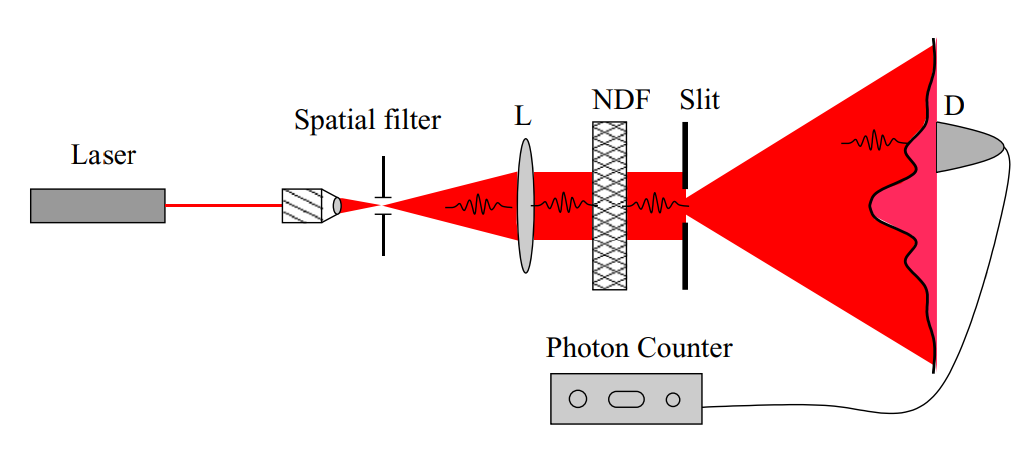
\includegraphics[width=0.8\textwidth]{Capitulo 8/Figuras/experimento.png}
        \caption{Configuración experimental.}
        \label{fig:experimento}
    \end{figure}
    
    Los resultados se verifican en un experimento de difracción con un haz láser ($\lambda$ $= 632$ $nm$) colimado con polarización lineal, el cual es atenuado mediante un arreglo de filtros de densidad neutra $(NDF)$ hasta contar un número limitado de fotones, y luego el haz es difractado por una rendija rectangular de $1905$ $\mu m$. La difracción se realiza en propagación en el espacio libre, a una distancia de $96,84$ $cm$ de la rendija hasta un contador de fotones del fotodiodo de avalancha $(D)$, cuyo diámetro es de $50$ $\mu m$. Los datos se toman durante un tiempo de $10$ $ms$ escaneando el campo difractado. \\
    
    El ajuste correcto entre los datos experimentales y el propagador de fotones según la ecuación ($\ref{eq:fresnelclasica}$) (ver Fig. $\ref{fig:dataexp}$) revela que la representación $q$ de un estado del campo puede usarse como guía para estudiar la propagación de fotones.
    
    
    \subsection{Simulación de la distribución de probabilidad para la propagación de fotones únicos}
    
    \begin{figure}[htbp]
        \centering    
        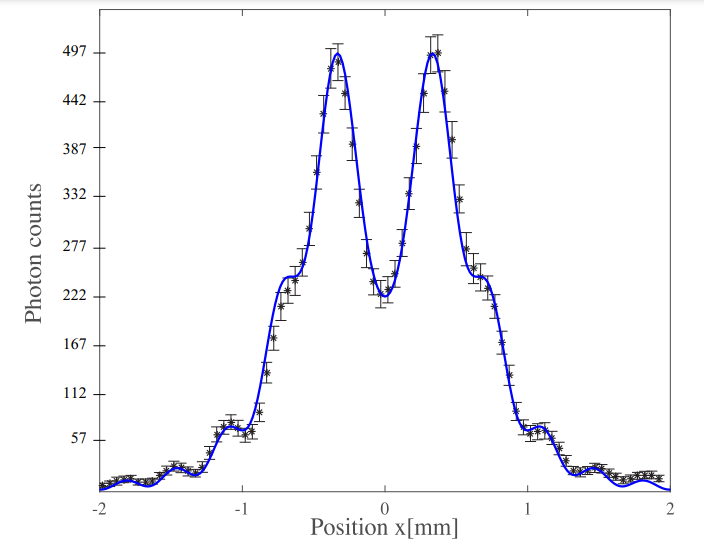
\includegraphics[width=0.7\textwidth]{Capitulo 8/Figuras/dataexp.png}
        \caption{Los datos experimentales se superpusieron a la curva azul que es la densidad de probabilidad normalizada, $\left | \Psi (x,z) \right |^{2}$, obtenido por simulación computacional.}
        \label{fig:dataexp}
    \end{figure}
    
    Es muy interesante explorar cómo evoluciona la distribución de densidad de probabilidad a medida que aumenta la distancia del plano de observación en el experimento de doble rendija. Aquí se muestra una simulación para varios planos de observación usando el propagador en Eq. ($\ref{eq:FRFT}$). A medida que el orden de la $FRFT$ se aproxima a $\alpha = \pi /2$, la distribución de densidad de probabilidad cambia hasta que alcanza el patrón de difracción de Fraunhofer característico, como se muestra en la Fig. $\ref{fig:simulacion}$. Este es un interferómetro de Young que utiliza haces gaussianos como fuentes con cintura $1/e^{2}$ radio de $0,6$ $mm$ y separación pico a pico de $4$ $mm$. Las densidades de distribución se trazan desde $\alpha = 0,8 \pi /2$ hasta $\alpha = \pi /2$ en relación con la distancia de propagación $z$.
    
    \begin{figure}[htbp]
        \centering    
        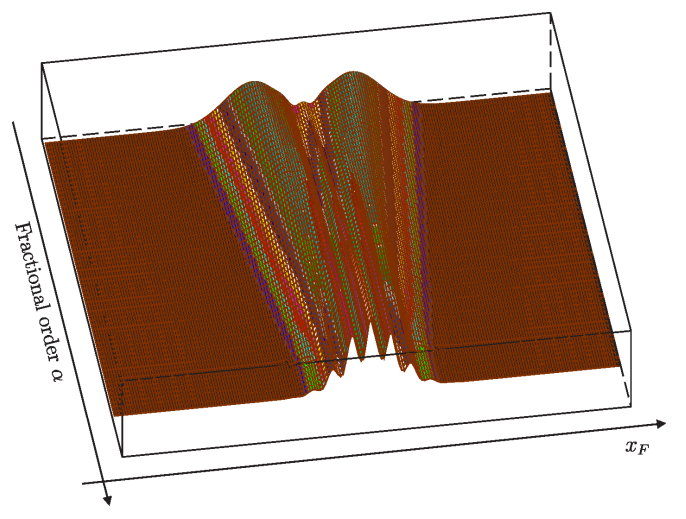
\includegraphics[width=0.7\textwidth]{Capitulo 8/Figuras/simulacion.png}
        \caption{Simulación de varias distribuciones de densidad de probabilidad a una distancia $z$.}
        \label{fig:simulacion}
    \end{figure}
    
    
    Aquí, el uso de la integral de difracción de Fresnel o, de manera equivalente, la transformada de Fourier fraccionaria ahora está fundamentalmente justificado para la propagación de un solo fotón. Nuestro tratamiento concuerda con las distribuciones de densidad de probabilidad encontradas experimentalmente por Kocsis et al. En el que pudieron construir trayectorias clásicas para fotones individuales en el interferómetro de doble rendija mediante una medición débil del momento sin destruir la interferencia. Es decir, la conclusión general, donde esas trayectorias representan el comportamiento promedio del conjunto de fotones, es confirmado por el resultado obtenido. \\
    
    Se ha encontrado un propagador de fotones que toma la forma de la integral de difracción de Fresnel clásica, mediante la estrecha conexión entre ambas y la transformada fraccionaria de Fourier. Se mostró que el observable $q$, debidamente escalado, corresponde a una posición observable transversal a la propagación del campo y paralela a la polarización del campo eléctrico. \\
    Esto significa que en el límite para un gran número de cuantos, la intensidad clásica del campo es entonces proporcional a la densidad de probabilidad, $|U(x,z)|^{2} \propto |\psi(q,t)|^{2}$, por lo que se satisface el principio de correspondencia, como se muestra en el experimento de conteo de fotones.